\section{Технический проект}
\subsection{Общая характеристика организации решения задачи}

Необходимо спроектировать и разработать web сервис, который реализует необходимый функционал фриланс-биржи для взаимодействия заказчика и исполнителя.

Web сервис представляет собой набор взаимосвязанных электронных страниц, которые сгруппированы по разделам, содержащие текстовую и графическую информацию. Сайт располагается в Интернете по определенному адресу – доменному имени сайта в виде www.имя\_сайта.ru. Каждая страница web-сайта – это текстовый документ, написанный на языке программирования (HTML, CSS, JavaScript и т.д.).

\subsubsection{Описание используемых технологий и языков программирования}

В процессе разработки проекта используются следующие технологии:

\begin{enumerate}
	\item Backend-часть: язык программирования Python, фреймворк Django, библиотека psycopg2 для взаимодействия с БД, СУБД PostgreSQL.
	\item Frontend-часть: языки программирования TypeScript, HTML, CSS и фреймворк Vue.js.
\end{enumerate}

\subsubsection{Backend-часть сервиса}

Backend-часть любого сервиса -- это, прежде всего, "<мозги"> всего сервиса. Через неё проходит вся логика работы приложения и взаимодействие с необходимыми данными. 

\paragraph{Язык программирования Python}

Python -- это язык прграммирования высокого уровня общего назначения с динамической строгой типизацией и автоматическим управлением памятью. Данный язык программирования достаточно универсален -- он может использоваться для таких задач, как разработка нейросетей, атоматизация тестирования, разработка игр и разработка web-приложений. Достигается такая гибкость благодаря различным библиотекам, которые создаются сообществом неравнодушных к языку пользователей.

\paragraph{Фреймворк Django}

Фреймворк Django -- это фреймворк для создания web-приложений, использующий шаблон проектирования MVC (Model-View-Controller). Состоит сайт на Django из одного или нескольких приложений, которые рекомендуется разрабатывать отчуждаемыми и подключаемыми. Работает фреймворк с множеством различных СУБД (в том числе и PostgreSQL). Из преимуществ так же можно выделить, что у Django присутствует собственный web-сервер, предназначенный для разработки -- он автоматически определяет изменения в файлах исходного кода и при нахождении таковых перезапускается, что в разы ускоряет разработку, но работает web-сервер в однопоточном режиме, потому он и предназначен только для разработки.

Так же можно выделить в данном фреймворке инструмент Django REST Framework, с помощью которого можно создать RESTful API. А API -- это свод определённых правил, по которым клиент общается с сервером, то есть сервер говорит, что он отдаёт необходимую информацию, если ему прислать определённые данные, если же отдать невалидные данные, то сервер их не примет и отдаст ошибку. Посредством API чаще всего происходит "<общение"> frontend-части сайта с его backend-частью, но так же используется для сторонних разработчиков, что бы они могли создавать, например, свои версии моильных приложений web-сервиса или какие-либо полезные скрипты (как пример - "<Вконтакте"> предоставляет подобные инструменты). 

\paragraph{Библиотека psycopg2}

Psycopg2 -- это наиболее популярный адаптер PostgreSQL для Python, в котором реализуется стандарт DB-API 2.0, который заключается в том, что бы у всех библиотек, которые выполняют взаимодействие с базой даннных, был единый интерфейс для работы с ними. Данная библиотека была выбрана не случайно -- она очень хорошо подходит для разработки web-сервиса, ведь она интегрируется с фреймворками создания web-приложений (Django, Flask), позволяя эффективно выполнять CRUD-операции, управлять транзакциями и работать с сложными типами данных. Так же данная библиотека отвечает требованиям безопасности со своим экранированием параметров запроса, что защищает от SQL-инъекций.

\paragraph{СУБД PostgreSQL} 

PostgreSQL -- это свободная объектно-реляционная СУБД. Она, исходя из названия, базируется на языке SQL и помогает в работе с базами данных. Их сильных сторон данной СУБД можно выделить высокопроизводительные механизмы транзакций, расширяемая система встроенных ЯП, возможность индексирования и расширяемость. 

\subsubsection{Frontend-часть сервиса}

Frontend-часть любого сервиса -- это то, с чем уже взаимодействует конечный пользователь. Здесь происходит графическое отображение элементов, необходимых для удобного взаимодействия пользователя с функционалом сервиса. Она являктся этакой прослойкой между пользователем и Backend-частью ("<мозгами">) сайта.

\paragraph{Язык программирования TypeScript}

TypeScript – объектно-ориентированный язык программирования для написания сценариев. По сути, TypeScript является надстройкой над JavaScript, расширяя возможности второго, ведь здесь даже есть возможность скомпилироваться обратно в JavaScript. А отличается он тем, что здесь есть возможность явного статического назначения типов, использования полноценных классов и подключения модулей. Используется TypeScript обычно для написания сценариев работы с web-страницами, отображаемыми web-браузером. Web-бра\-у\-зер интерпретирует код сценария языка TypeScript, и на основе описанных в сценарии действий производит манипуляции с разметкой web-страницы. Посредством языка TypeScript реализуется возможность программирования на стороне клиента. 

\paragraph{Языки разметки HTML и CSS}

HTML (HyperText Markup Language) -- это язык гипертекстовой разметки документов, предназначенный для просмотра web-страниц при помощи браузера. Код таких документов браузером интерпретируются в интерфейс, который отображается на экране монитора. Состоит данный документ обычно из тегов - сначала идёт тег head в котором обычно определяются настройки документа, а после идёт тег body, в котором и заключается вся отображаемая информация. 

CSS (Cascading Style Sheets) -- это язык декорирования и описания внешнего вида документов (обычно используется для HTML-документов). Состоит данный файл из селекторов, в которых перечисляются их свойства и заданные для них значения. В большинстве ситуаций HTML и CSS идут неразрывно рука об руку -- с помощью CSS задаётся внешний вид элементов, указанных в HTML-документе.

\paragraph{Фреймворк Vue.js}

Vue.js -- это opensource JS-фреймворк, предназначенный для создания пользовательских интерфейсов. Из явных преимуществ можно выделить, что его не сложно освоить и легко интегрировать в проекты с использованием других JS-библиотек. Используется здесь компонентный подход, что позволяет разбивать интерфейс на переиспользуемые блоки, а его свойство реактивности автоматически обновляет DOM при изменении данных. Достигаются все преимущества с помощью встроенных инструментов: VueRouter для маршрутизации, Vuex для управления состоянием и CompositionAPI для лучшей организации кода.

\subsection{Компоненты программной системы}

Диаграмма компонентов описывает особенности физического представления разрабатываемой системы. Она позволяет определить архитектуру системы, установив зависимости между программными компонентами, в роли которых может выступать как исходный, так и исполняемый код. Основными графическими элементами диаграммы компонентов являются компоненты, интерфейсы, а также зависимости между ними. На рисунке \ref{comp:image} изображена диаграмма компонентов для проектируемой системы.

\begin{figure}[ht]
	\center{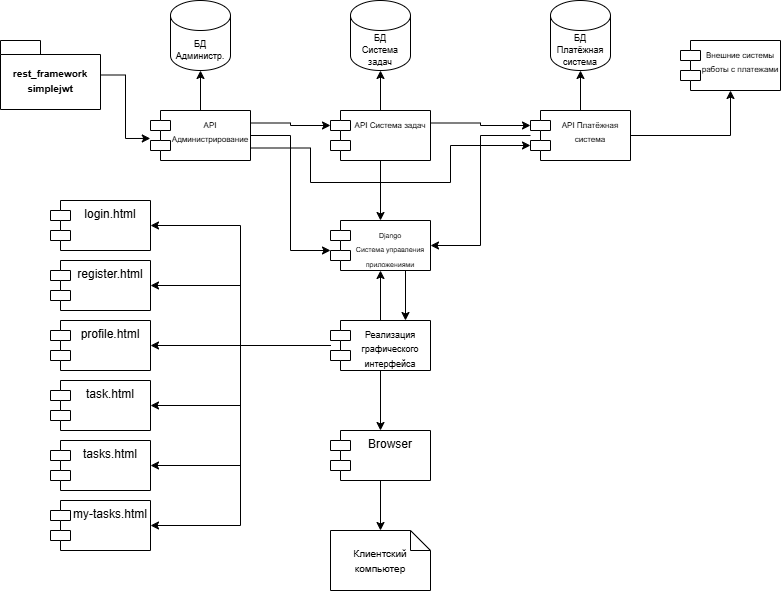
\includegraphics[width=1\linewidth]{components.png}}
	\caption{Диаграмма компонентов}
	\label{comp:image}
\end{figure}

Компненты БД являются базами данных, которые созданы отдельно для каждой подсистемы.

Компонент "<API Администрирование"> отвечает за работу с сущностями пользователей и их авторизацию. Для реализации авторизации используется библиотека simplejwt из пакета rest\_framework. Взаимодействие предусмотрено с подсистемами "<Система задач"> и "<Платёжная система">.

Компонент "<API Система задач"> отвечает за работу с сущностями задач.  Взаимодействие предусмотрено с подсистемами "<Администрирование"> для проверки авторизации в взаимодействия с польхователями и "<Платёжная система"> для получения на задачу средств и дальнейшем переводе их на виртуальный счёт исполнителя.

Компонент "<API Платёжная система"> отвечает за работу с сущностями платежей и платёжных транзакция. Взаимодействие предусмотрено с подсистемами "<Система задач"> для платежей, связанных с задачами, "<Администрирование"> для платежей, связанных с пользователями и внешними системами работы с платежами для пополнения виртуального счёта и вывода средств с него.

Компонент "<Django Система управления приложениями"> является связующим звеном между графическим интерфейсом и API взаимодействующих с ним подсистем. Через него идёт запуск сервера и вызов методов для размещения или получения информации.

Компонент "<Реализация графического интерфейса"> отвечает за отправку отображения графического интерфейса клиенту посредством отправки HTML-документа, который уже расшифровывает компонент "<Browser">. Данные, которые отображаются в HTML-документе, подтягиваются с backend-части при взаимодействии с компонентом "<Django Система управления приложениями"> через отправку запросов к API необходимой подсистемы. 

\subsection{Проект данных программной системы}

Исходя из требований технического задания, программно информационная система должна взаимодействовать с тремя базами данных. Для разработки сервиса требуется использовать СУБД PostgreSQL.

Во-первых, данная СУБД предоставляет надёжную и отказоустойчивую систему хранения данных, что очень важно для платформы, работающей с транзакциями и персональными данными пользователей.

Во-вторых, PostgreSQL показывает свою производительность путём эффективной работы с индексами, что в разы ускоряет поиск задач. Встроенный планировщик запросов оптимизирует выполнение сложных запросов, таких как выборка задач с учетом множества условий.

Третье её преимущество - лёгкая масштабируемость вместе с ростом сервиса. Поддержка табличных пространств позволяет распределять нагрузку по дискам, а механизмы секционирования помогают управлять большими таблицами.

\subsubsection{Описание сущностей клиентской части}

В состав сущностей "<Авторизационные данные">, "<Заказчик">, "<Исполнитель">, "<Задача">, "<Статус задачи">, "<Отклик на задачу">, "<Виртуальный счёт"> и "<История операций">, можно включить атрибуты, представленные в таблицах \ref{login:table} -- \ref{payment:table} соответственно.

\begin{xltabular}{\textwidth}{|l|l|p{1.7cm}|X|}
	\caption{Атрибуты сущности "<Авторизационные данные">\label{login:table}}\\ \hline
	\centrow Поле & \centrow Тип & \centrow Обяза\-тельное & \centrow Описание \\ \hline
	\thead{1} & \thead{2} & \centrow 3 & \centrow 4 \\ \hline
	\endfirsthead
	\continuecaption{Продолжение таблицы \ref{login:table}}
	\thead{1} & \thead{2} & \centrow 3 & \centrow 4 \\ \hline
	\finishhead
	user\_id & integer & + & Уникальный идентификатор пользователя \\ \hline 
	login & character varying & + & Логин пользователя \\ \hline 
	password & character varying & + & Пароль пользователя \\ \hline 
	user\_role & character varying & + & Роль пользователя \\ \hline 
	create\_dttm & date & + & Дата создания аккаунта \\ \hline
\end{xltabular}

\begin{xltabular}{\textwidth}{|l|l|p{1.7cm}|X|}
	\caption{Атрибуты сущности "<Заказчик">\label{employer:table}}\\ \hline
	\centrow Поле & \centrow Тип & \centrow Обяза\-тельное & \centrow Описание \\ \hline
	\thead{1} & \thead{2} & \centrow 3 & \centrow 4 \\ \hline
	\endfirsthead
	\continuecaption{Продолжение таблицы \ref{employer:table}}
	\thead{1} & \thead{2} & \centrow 3 & \centrow 4 \\ \hline
	\finishhead
	user\_id & integer & + & Уникальный идентификатор пользователя \\ \hline 
	name & character varying & + & Имя заказчика \\ \hline 
	organization & character varying & + & Организация, от которой представлен заказчик \\ \hline 
	description & character varying & - & Описание заказчика \\ \hline 
	create\_dttm & date & + & Дата создания аккаунта 
\end{xltabular}

\begin{xltabular}{\textwidth}{|l|l|p{1.7cm}|X|}
	\caption{Атрибуты сущности "<Исполнитель">\label{executor:table}}\\ \hline
	\centrow Поле & \centrow Тип & \centrow Обяза\-тельное & \centrow Описание \\ \hline
	\thead{1} & \thead{2} & \centrow 3 & \centrow 4 \\ \hline
	\endfirsthead
	\continuecaption{Продолжение таблицы \ref{executor:table}}
	\thead{1} & \thead{2} & \centrow 3 & \centrow 4 \\ \hline
	\finishhead
	user\_id & integer & + & Уникальный идентификатор пользователя \\ \hline 
	name & character varying & + & Имя исполнителя \\ \hline 
	description & character varying & - & Описание исполнителя \\ \hline
	level & integer & + & Уровень исполнителя \\ \hline  
	level\_exp & integer & + & Опыт в пределах уровня исполнителя \\ \hline  
	loyality & integer & + & Рейтинг исполнителя \\ \hline  
	create\_dttm & date & + & Дата создания аккаунта 
\end{xltabular}

\begin{xltabular}{\textwidth}{|l|l|p{1.7cm}|X|}
	\caption{Атрибуты сущности "<Задача">\label{task:table}}\\ \hline
	\centrow Поле & \centrow Тип & \centrow Обяза\-тельное & \centrow Описание \\ \hline
	\thead{1} & \thead{2} & \centrow 3 & \centrow 4 \\ \hline
	\endfirsthead
	\continuecaption{Продолжение таблицы \ref{task:table}}
	\thead{1} & \thead{2} & \centrow 3 & \centrow 4 \\ \hline
	\finishhead
	task\_id & integer & + & Уникальный идентификатор задачи \\ \hline 
	task\_initiator & integer & + & Идентификатор пользователя, создавшего задачу \\ \hline 
	task\_name & character varying & + & Название задачи \\ \hline 
	task\_desc & character varying & - & Описание задачи \\ \hline 
	cost & double precision & + & Стоимость задачи \\ \hline  
	complexity & integer & + & Сложность задачи 
\end{xltabular}

\begin{xltabular}{\textwidth}{|l|l|p{1.7cm}|X|}
	\caption{Атрибуты сущности "<Статус задачи">\label{status:table}}\\ \hline
	\centrow Поле & \centrow Тип & \centrow Обяза\-тельное & \centrow Описание \\ \hline
	\thead{1} & \thead{2} & \centrow 3 & \centrow 4 \\ \hline
	\endfirsthead
	\continuecaption{Продолжение таблицы \ref{status:table}}
	\thead{1} & \thead{2} & \centrow 3 & \centrow 4 \\ \hline
	\finishhead
	task\_id & integer & + & Уникальный идентификатор задачи \\ \hline 
	task\_status & character varying & + & Статус задачи \\ \hline 
	executor\_id & integer & - & Идентификатор назначенного исполнителя \\ \hline 
	create\_dttm & date & + & Дата создания задачи \\ \hline 
	modify\_dttm & date & + & Дата изменения задачи \\ \hline  
	end\_dttm & date & - & Дата завершения задачи
\end{xltabular}

\begin{xltabular}{\textwidth}{|l|l|p{1.7cm}|X|}
	\caption{Атрибуты сущности "<Отклик на задачу">\label{vote:table}}\\ \hline
	\centrow Поле & \centrow Тип & \centrow Обяза\-тельное & \centrow Описание \\ \hline
	\thead{1} & \thead{2} & \centrow 3 & \centrow 4 \\ \hline
	\endfirsthead
	\continuecaption{Продолжение таблицы \ref{vote:table}}
	\thead{1} & \thead{2} & \centrow 3 & \centrow 4 \\ \hline
	\finishhead
	task\_id & integer & + & Уникальный идентификатор задачи \\ \hline 
	executor\_id & integer & + & Идентификатор назначенного исполнителя \\ \hline 
	vote\_dttm & date & + & Дата отклика \\ \hline 
	is\_refund & boolean & + & Был ли отменён отклик 
\end{xltabular}

\begin{xltabular}{\textwidth}{|l|l|p{1.7cm}|X|}
	\caption{Атрибуты сущности "<Виртуальный счёт">\label{pacc:table}}\\ \hline
	\centrow Поле & \centrow Тип & \centrow Обяза\-тельное & \centrow Описание \\ \hline
	\thead{1} & \thead{2} & \centrow 3 & \centrow 4 \\ \hline
	\endfirsthead
	\continuecaption{Продолжение таблицы \ref{pacc:table}}
	\thead{1} & \thead{2} & \centrow 3 & \centrow 4 \\ \hline
	\finishhead
	card\_id & integer & + & Уникальный идентификатор виртуального счёта \\ \hline 
	owner\_id & integer & + & Идентификатор владельца счёта \\ \hline 
	role & character varying & + & Роль владельца счёта \\ \hline 
	balance & double precision & + & Баланс средств на счёте \\ \hline 
	create\_dttm & date & + & Дата создания счёта 
\end{xltabular}

\begin{xltabular}{\textwidth}{|l|l|p{1.7cm}|X|}
	\caption{Атрибуты сущности "<История операций">\label{payment:table}}\\ \hline
	\centrow Поле & \centrow Тип & \centrow Обяза\-тельное & \centrow Описание \\ \hline
	\thead{1} & \thead{2} & \centrow 3 & \centrow 4 \\ \hline
	\endfirsthead
	\continuecaption{Продолжение таблицы \ref{payment:table}}
	\thead{1} & \thead{2} & \centrow 3 & \centrow 4 \\ \hline
	\finishhead
	payment\_id & integer & + & Уникальный идентификатор платежа \\ \hline 
	receiver\_id & integer & + & Идентификатор получателя платежа \\ \hline 
	initiator & integer & - & Идентификатор инициатора платежа \\ \hline 
	task\_id & integer & - & Идентификатор задачи, за которую был совершён платёж \\ \hline
	payment\_count & double precision & + & Сумма операции \\ \hline 
	payment\_dttm & date & + & Дата платежа
\end{xltabular}

\subsection{Проектирование пользовательского интерфейса}

На основании требований к пользовательскому интерфейсу, представленных в пункте 2.3.3 технического задания, был разработан графический интерфейс web-сервиса. Для создания интерфейса используется HTML-разметка с использованием CSS-стилей и JavaScript-фреймворком Vue.js.

На рисунке \ref{m1:image} представлен макет интерфейса страницы "<Страница входа">. Макет содержит следующие элементы:

\begin{enumerate}
	\item Поле для ввода логина.
	\item Поле для ввода пароля.
	\item Кнопка входа пользователя на сервис.
	\item Кнопка регистрации пользователя.
	\item Кнопка восстановления пароля.
\end{enumerate}
\clearpage

\begin{figure}[ht]
	\center{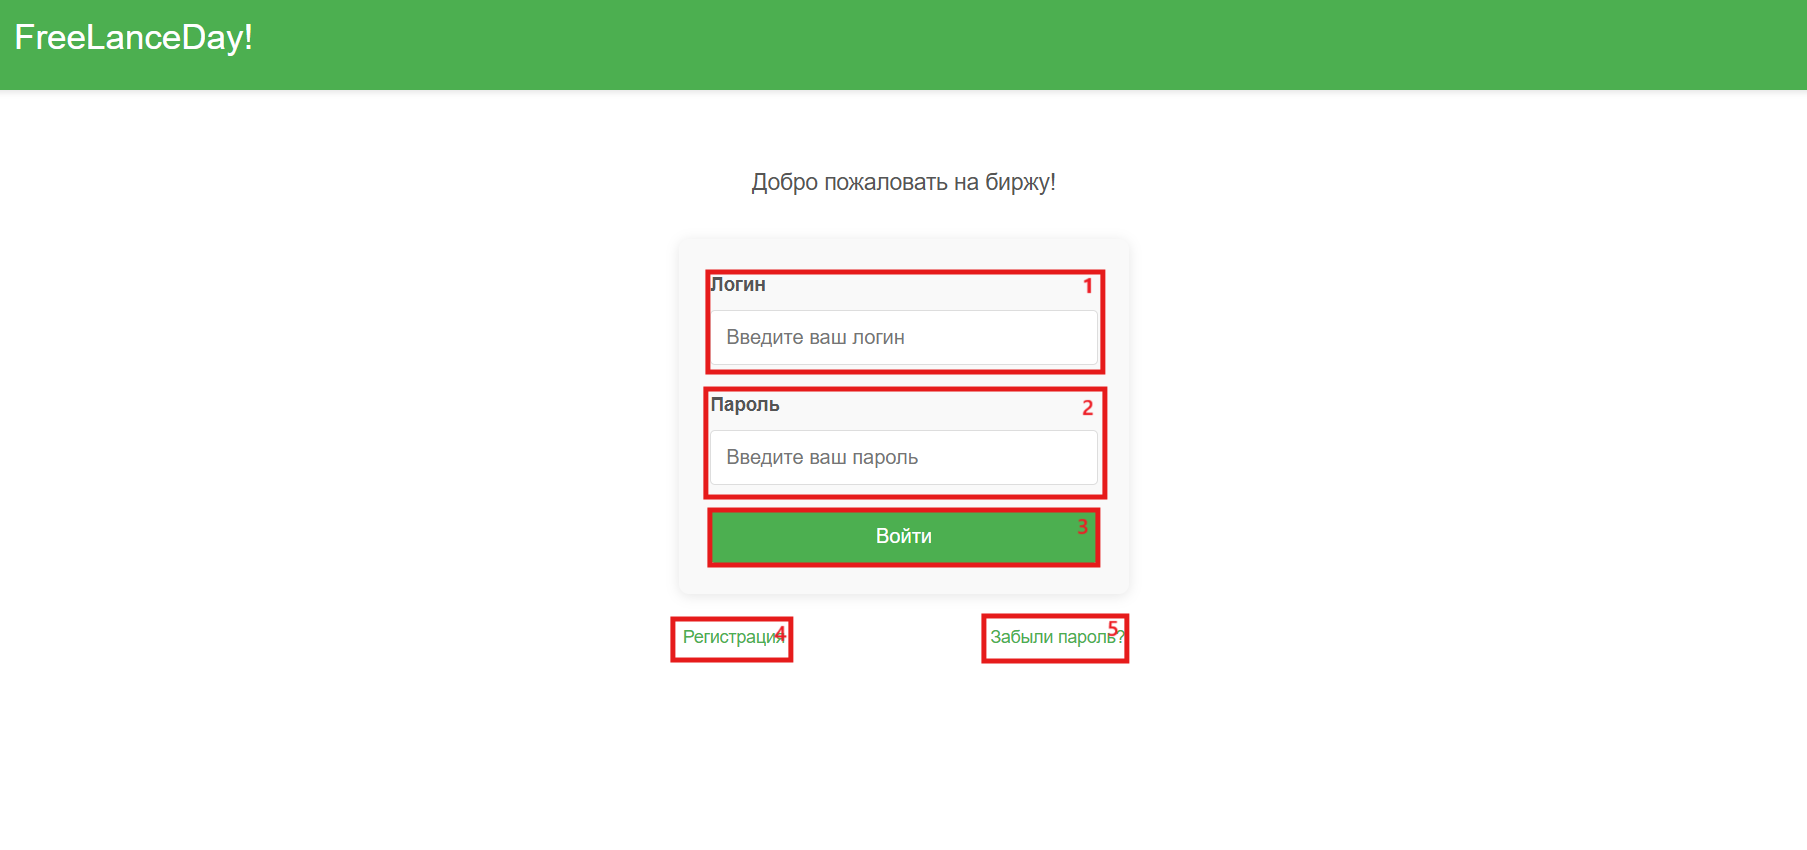
\includegraphics[width=1\linewidth]{maket1.png}}
	\caption{Макет страницы "<Страница входа">}
	\label{m1:image}
\end{figure}

На рисунке \ref{m2:image} представлен макет интерфейса страницы "<Создание задачи">. Макет содержит следующие элементы:

\begin{enumerate}
	\item Кнопка перехода в профиль авторизованного пользователя.
	\item Кнопка перехода к задачам авторизованного пользователя.
	\item Кнопка перехода к просмотру баланса авторизованного пользователя.
	\item Логин авторизованного пользователя.
	\item Кнопка выхода из аккаунта.
	\item Поле для ввода названия задачи.
	\item Поле для ввода описания задачи.
	\item Поле для ввода стоимости задачи.
	\item Выпадающий список для выбора сложности задачи.
	\item Кнопка отмены создания задачи.
	\item Кнопка создания задачи (неактивна).
\end{enumerate}
\clearpage

\begin{figure}[ht]
	\center{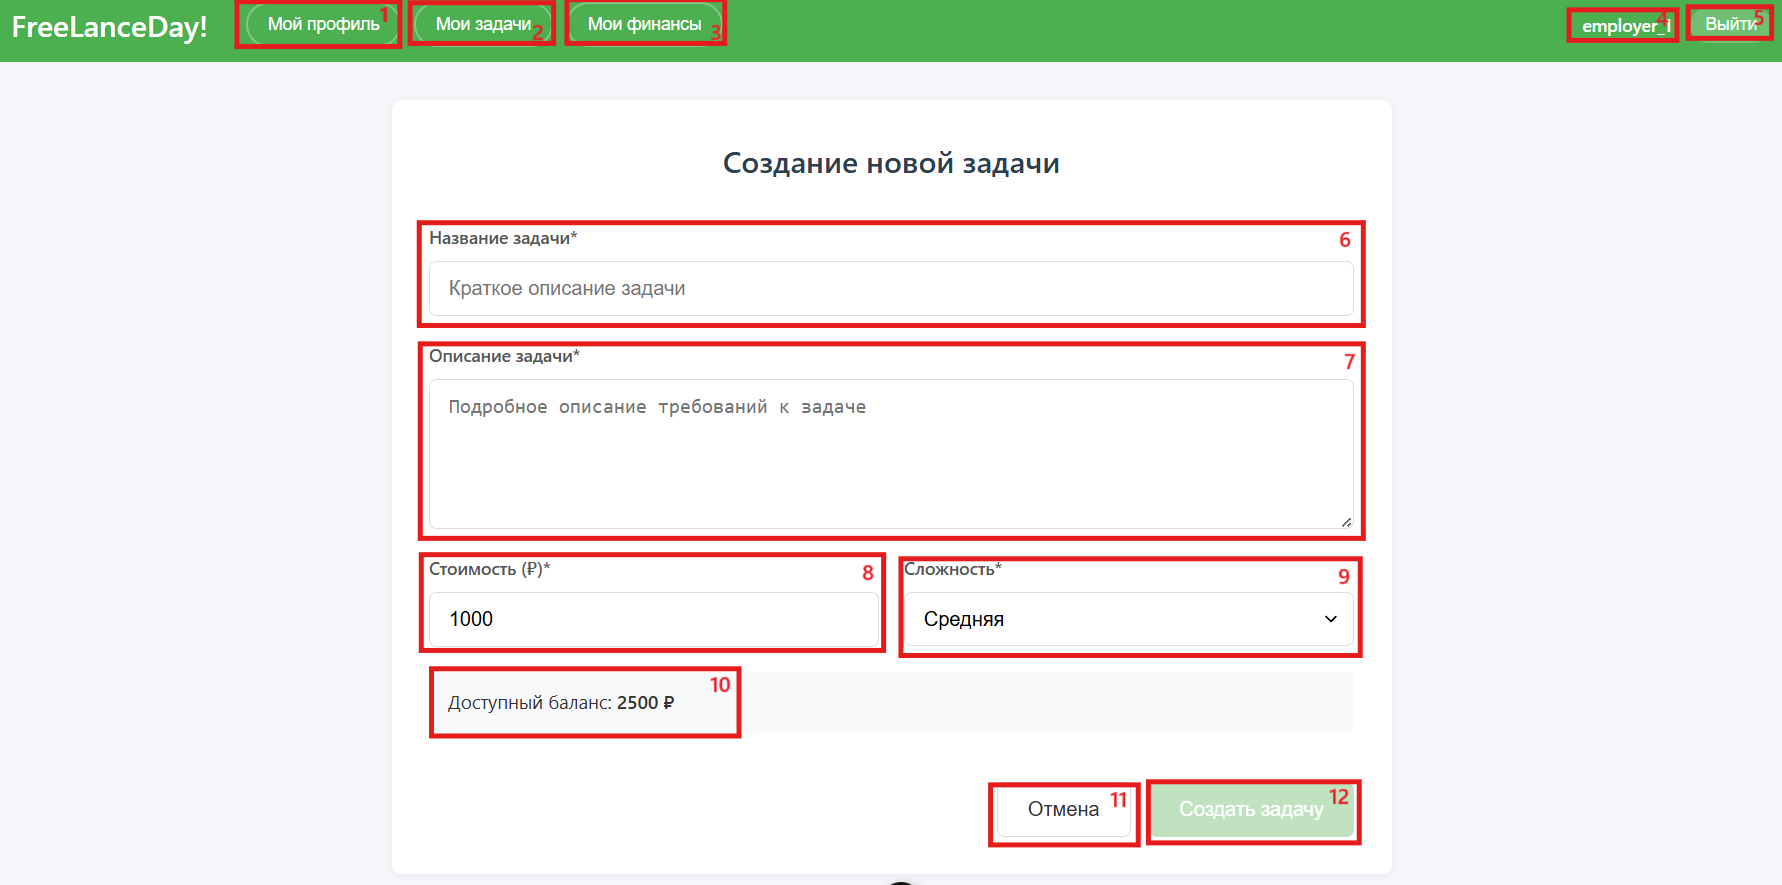
\includegraphics[width=1\linewidth]{maket2.png}}
	\caption{Макет страницы "<Создание задачи">}
	\label{m2:image}
\end{figure}

На рисунке \ref{m3:image} представлен макет интерфейса страницы "<Просмотр задач">. Макет содержит следующие элементы:

\begin{enumerate}
	\item Кнопка перехода в профиль авторизованного пользователя.
	\item Кнопка перехода к просмотру баланса авторизованного пользователя.
	\item Кнопка перехода к созданию задачи.
	\item Логин авторизованного пользователя.
	\item Кнопка выхода из аккаунта.
	\item Блок информации о задаче.
	\item Название задачи.
	\item Описание задачи.
	\item Стоимость задачи.
	\item Кнопка перехода к подробному описанию задачи.
\end{enumerate}
\clearpage

\begin{figure}[ht]
	\center{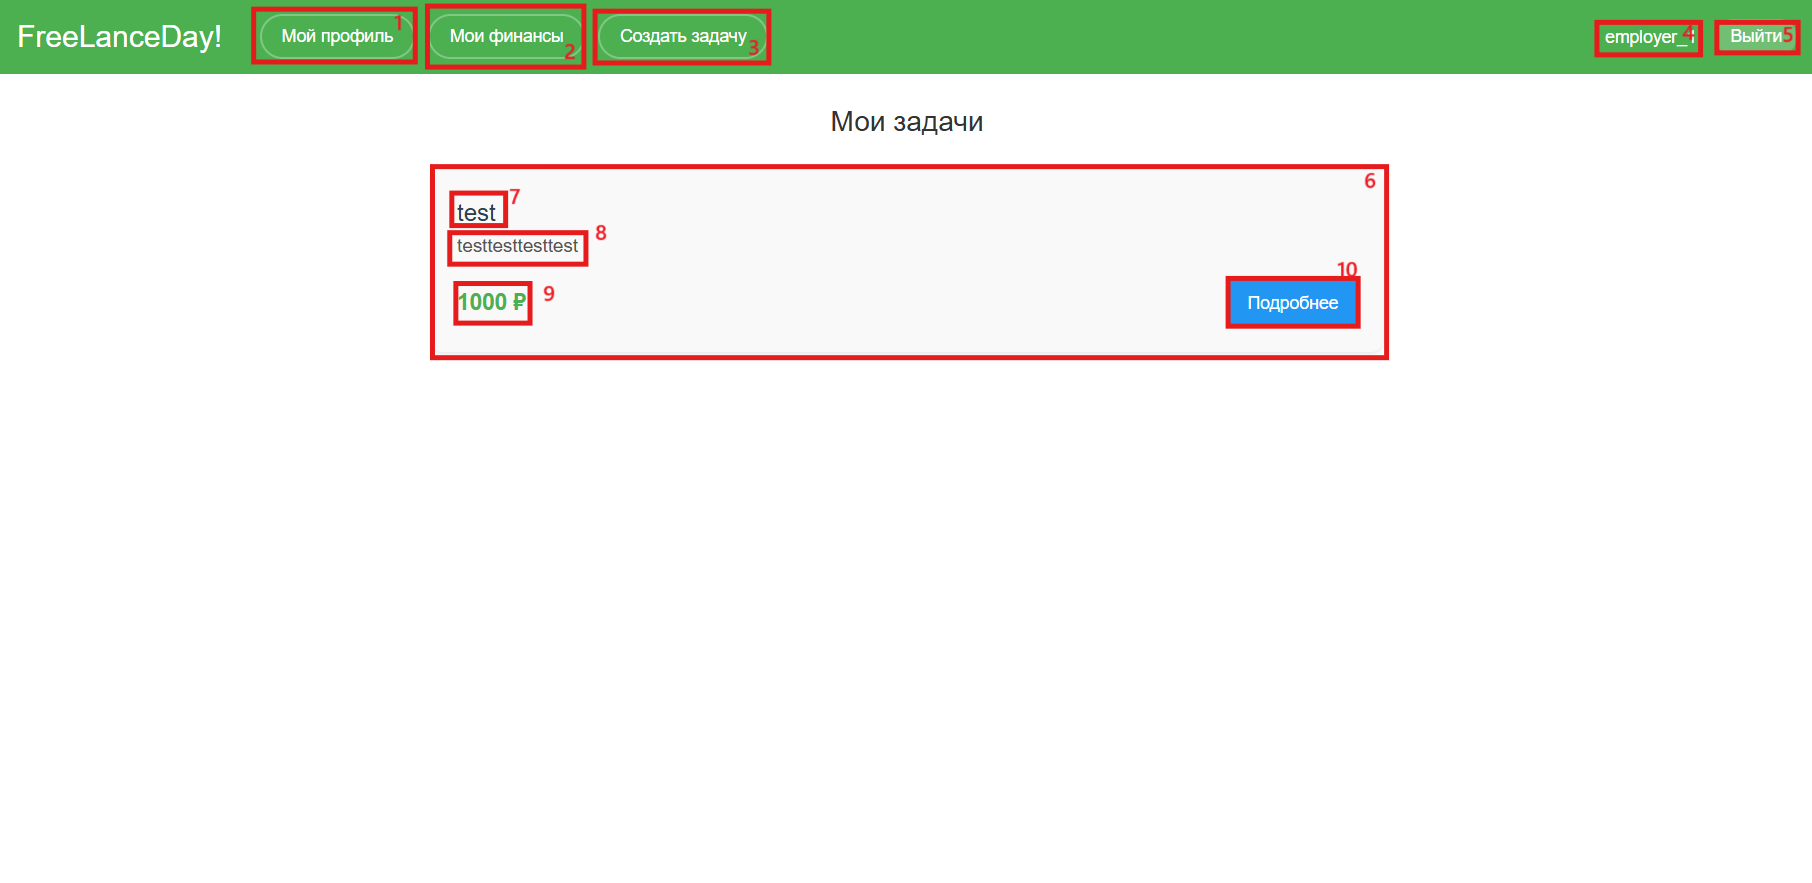
\includegraphics[width=1\linewidth]{maket3.png}}
	\caption{Макет страницы "<Просмотр задач">}
	\label{m3:image}
\end{figure}

На рисунке \ref{m4:image} представлен макет интерфейса страницы "<Просмотр баланса виртуального счёта">. Макет содержит следующие элементы:

\begin{enumerate}
	\item Кнопка перехода в профиль авторизованного пользователя.
	\item Кнопка перехода к задачам авторизованного пользователя.
	\item Кнопка перехода к созданию задачи.
	\item Логин авторизованного пользователя.
	\item Кнопка выхода из аккаунта.
	\item Баланс виртуального счёта авторизованного пользователя.
	\item Кнопка перехода к странице пополнения баланса.
	\item Блок истории операций.
	\item Блок информации о транзакции.
	\item Сумма транзакции.
	\item Тип транзакции.
	\item Описание транзакции.
	\item Дата транзакции.
\end{enumerate}
\clearpage

\begin{figure}[ht]
	\center{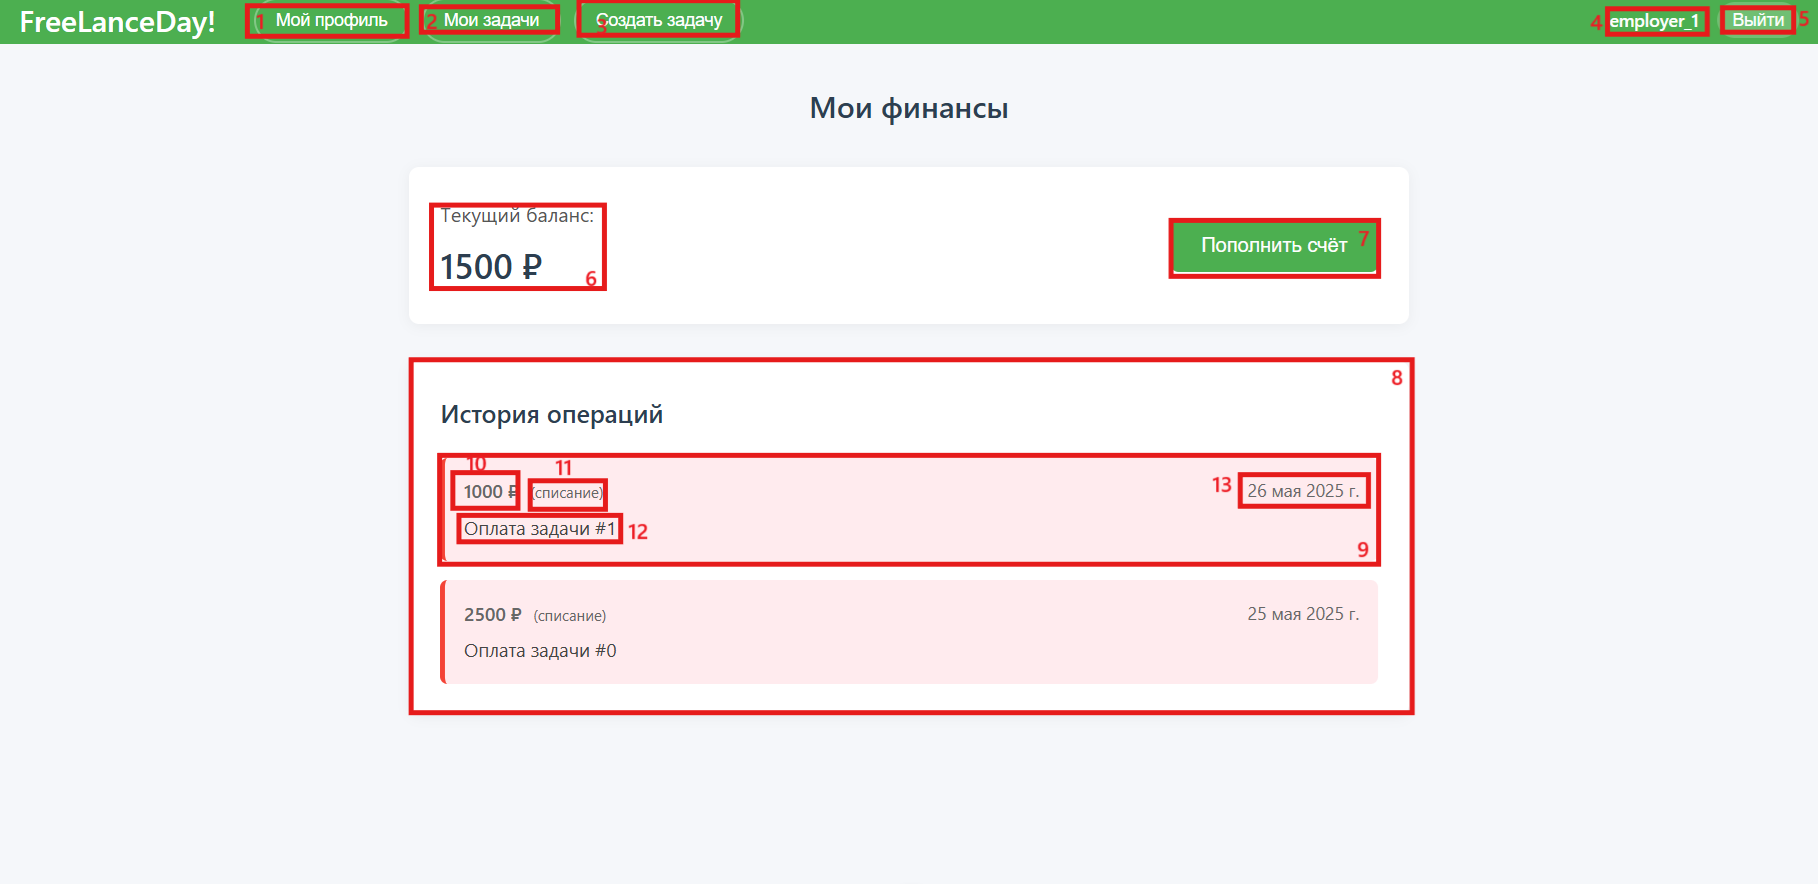
\includegraphics[width=1\linewidth]{maket4.png}}
	\caption{Макет страницы "<Просмотр баланса виртуального счёта">}
	\label{m4:image}
\end{figure}

На рисунке \ref{m5:image} представлен макет интерфейса страницы "<Просмотр профиля авторизованного пользователя">. Макет содержит следующие элементы:

\begin{enumerate}
	\item Кнопка перехода к задачам авторизованного пользователя.
	\item Кнопка перехода к просмотру баланса авторизованного пользователя.
	\item Кнопка перехода к созданию задачи.
	\item Логин авторизованного пользователя.
	\item Кнопка выхода из аккаунта.
	\item Дата создания аккаунта.
	\item Блок основной информации о пользователе.
	\item Имя пользователя.
	\item Организация пользователя.
	\item Описание пользователя.
	\item Кнопка перехода к редактированию профиля.
\end{enumerate}
\clearpage

\begin{figure}[ht]
	\center{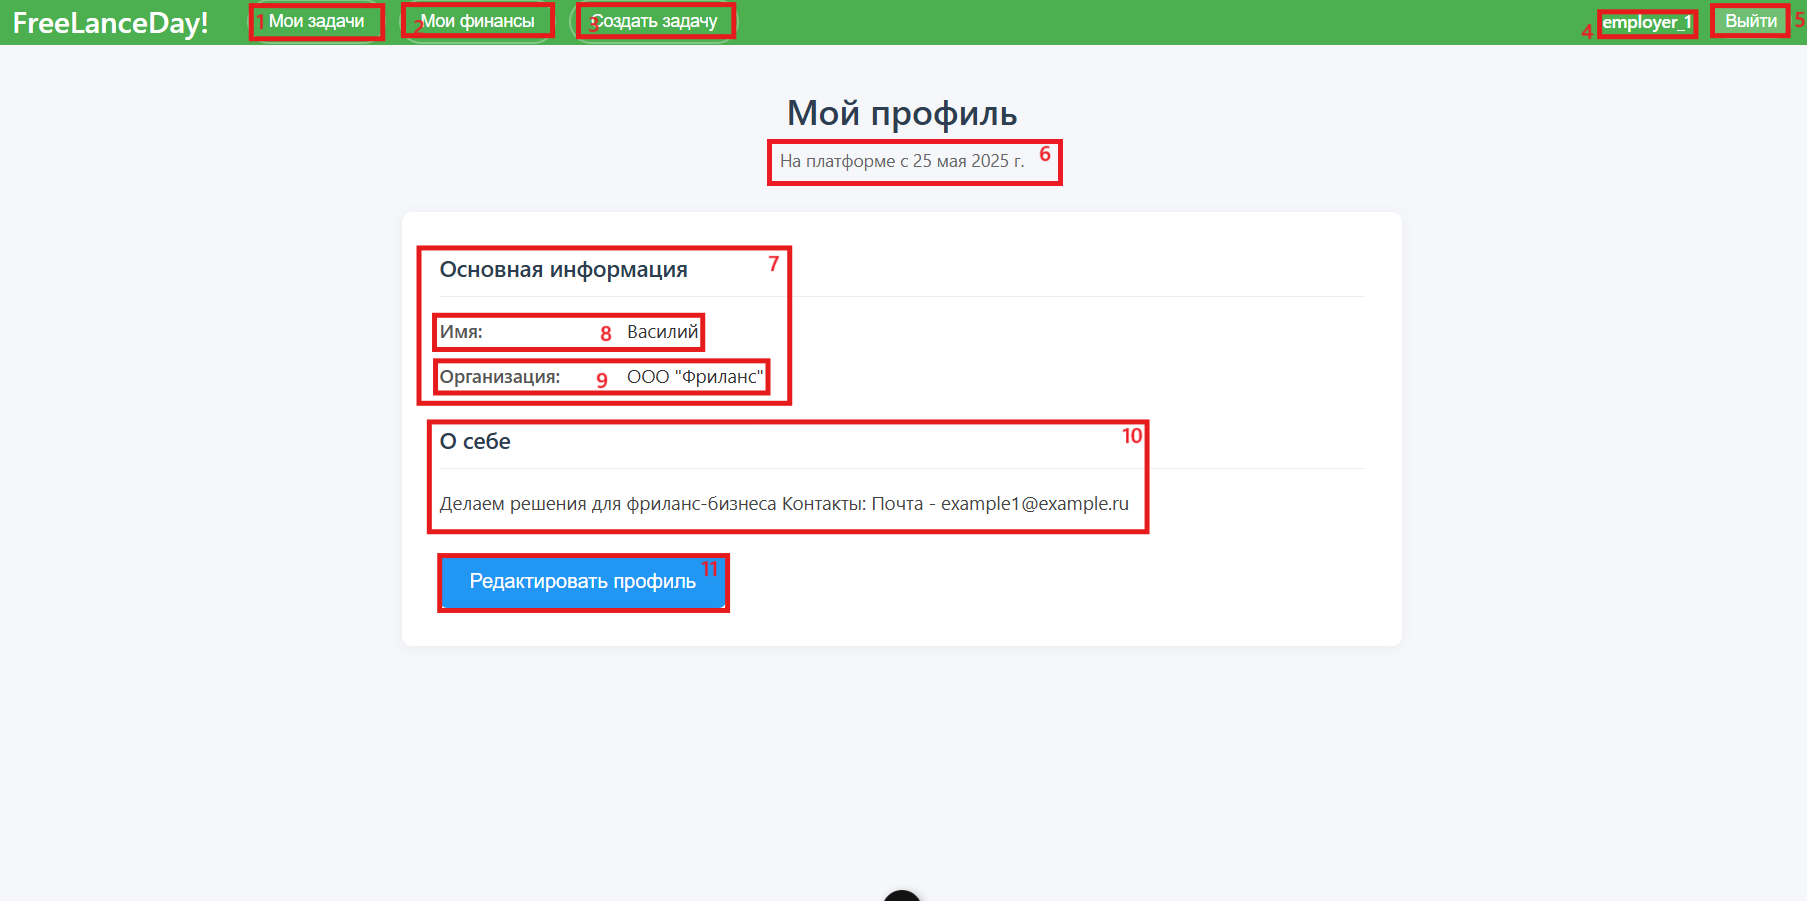
\includegraphics[width=1\linewidth]{maket5.png}}
	\caption{Макет страницы "<Просмотр профиля авторизованного пользователя">}
	\label{m5:image}
\end{figure}

На рисунке \ref{m6:image} представлен макет интерфейса страницы "<Пополнение виртуального счёта">. Макет содержит следующие элементы:

\begin{enumerate}
	\item Поле ввода суммы пополнения.
	\item Кнопки быстрого ввода суммы пополнения.
	\item Кнопки выбора способа оплаты.
	\item Поле ввода номера карты.
	\item Поле ввода срока действия карты.
	\item Поле ввода CVV/CVC кода карты.
	\item Кнопка пополнения счёта (неактивна).
\end{enumerate}
\clearpage

\begin{figure}[ht]
	\center{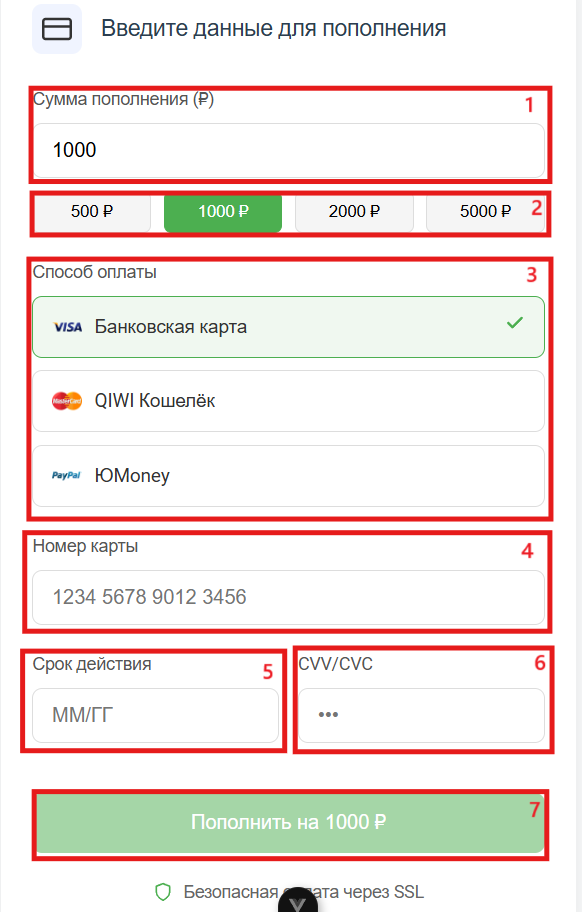
\includegraphics[width=0.7\linewidth]{maket6.png}}
	\caption{Макет страницы "<Пополнение виртуального счёта">}
	\label{m6:image}
\end{figure}

На рисунке \ref{m7:image} представлен макет интерфейса страницы "<Просмотр информации о задаче">. Макет содержит следующие элементы:

\begin{enumerate}
	\item Кнопка перехода в профиль авторизованного пользователя.
	\item Кнопка перехода к задачам авторизованного пользователя.
	\item Кнопка перехода к просмотру баланса авторизованного пользователя.
	\item Кнопка перехода к созданию задачи.
	\item Логин авторизованного пользователя.
	\item Кнопка выхода из аккаунта.
	\item Название задачи.
	\item Статус задачи.
	\item Стоимость задачи.
	\item Сложность задачи.
	\item Дата создания задачи.
	\item Заказчик, создавший задачу (ссылка на его профиль).
	\item Описание задачи.
	\item Кнопка перехода к просмотру откликов.
\end{enumerate}

\begin{figure}[ht]
	\center{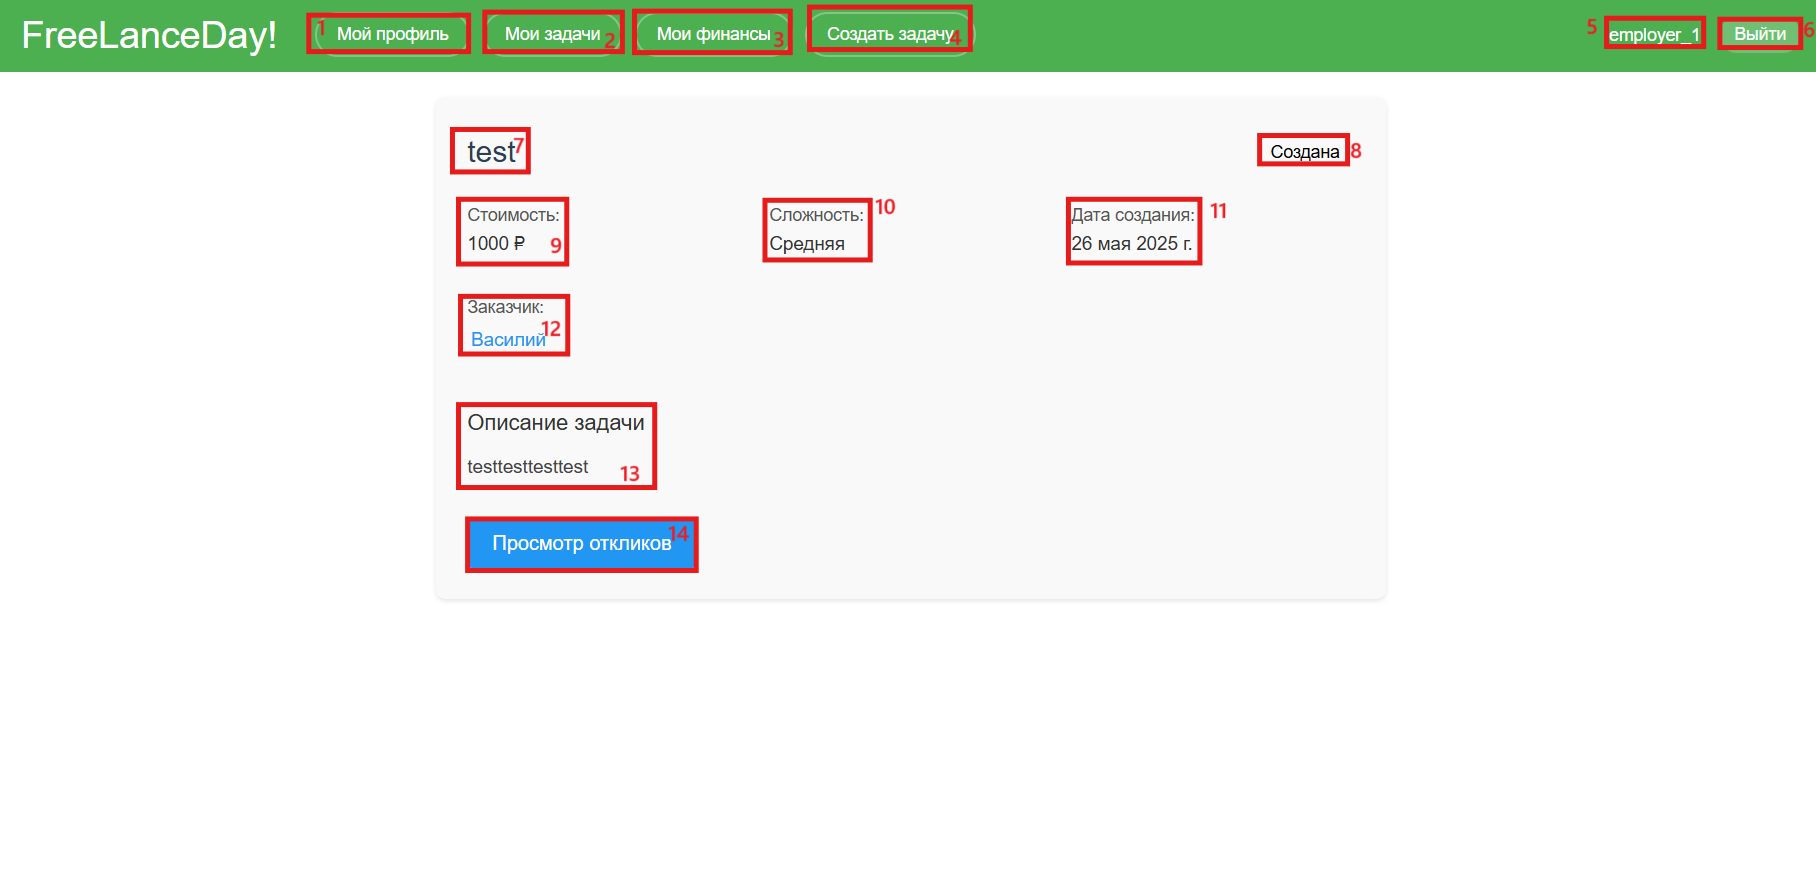
\includegraphics[width=1\linewidth]{maket7.png}}
	\caption{Макет страницы "<Просмотр информации о задаче">}
	\label{m7:image}
\end{figure}

На рисунке \ref{m8:image} представлен макет интерфейса страницы "<Просмотр откликов">. Макет содержит следующие элементы:

\begin{enumerate}
	\item Кнопка перехода в профиль авторизованного пользователя.
	\item Кнопка перехода к задачам авторизованного пользователя.
	\item Кнопка перехода к просмотру баланса авторизованного пользователя.
	\item Кнопка перехода к созданию задачи.
	\item Логин авторизованного пользователя.
	\item Кнопка выхода из аккаунта.
	\item Название страницы и название задачи, на котрую осуществляется просмотр откликов.
	\item Имя исполнителя (ссылка на его профиль).
	\item Уровень исполнителя.
	\item Уровень лояльности исполнителя.
	\item Кнопка назначения исполнителя на задачу.
	\item Дата регистрации исполнителя.
	\item Описание исполнителя.
\end{enumerate}

\begin{figure}[ht]
	\center{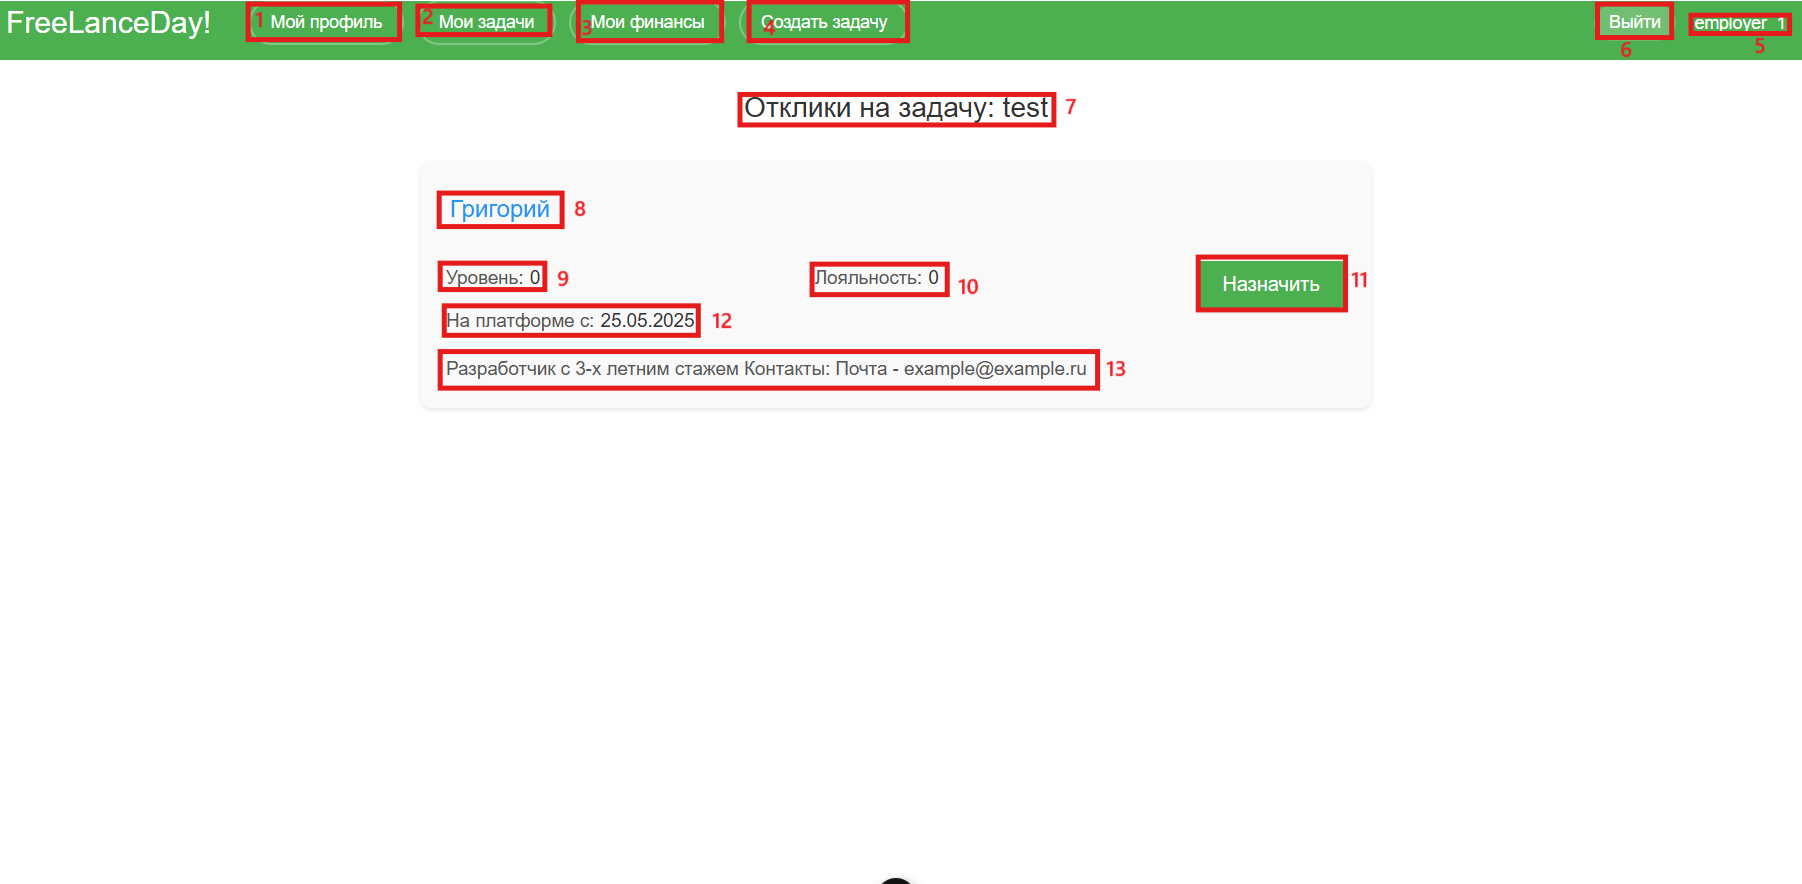
\includegraphics[width=1\linewidth]{maket8.png}}
	\caption{Макет страницы "<Просмотр откликов">}
	\label{m8:image}
\end{figure}